\chapter{Introduction}
\label{introduction}

\section{Modular Robots}
\label{introduction_intro}

Modular robots are robots composed by several autonomous units, called ``modules'', that work together in order to increase the overall capabilities of a single unit. Each module is a complete robot itself, having its own control electronics, actuators, sensors, power supply and some way of connecting to other modules to form a modular robot.\\

Modular robots have several advantages over traditional robots, the first being adaptability. Their modular design allows some modular robots to reconfigure themselves, changing the position of some of the modules within the robot body. This self-reconfiguration is very useful in unknown or changing environments, as the robot can adapt its body depending on the terrain, for example, becoming a snake-like robot to pass through pipes or holes, and later on reconfiguring to a legged robot to stand on top of obstacles. 
In some cases they can even detach themselves from the robot in order to explore the surroundings and act like a swarm, and then return back and reconstruct the robot again. Figure \ref{fig:intro_mtran3} shows the reconfiguration of a M-TRAN III modular robot from a quadruped configuration to a snake robot.\\

\begin{figure}[h]
		\centering
        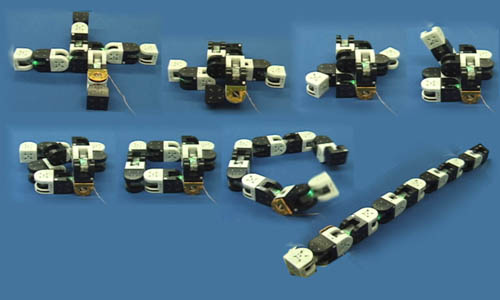
\includegraphics[width=0.6\textwidth]{images/Intro_mtran3.jpg}
        \caption{M-TRAN III modular robot reconfiguring from quadruped to snake robot.}
        \label{fig:intro_mtran3}
\end{figure} 


 In general, modular robots are used in applications in which the operating conditions of the robot are not known when the robot is to be designed, such as space exploration, battlefield reconnaissance, finding victims among the debris in natural catastrophes and other similar tasks involving complicated terrains.\\

As the robot does not rely on a single module, modular robots are fault-tolerant, and most of the robot functionality will remain even when some modules fail. Those bad-functioning modules can be substituted by other new modules, giving self-reconfigurable modular robots the property of self-repairing.\\

Modular robots can generally be classified by the arrangement of their basic unit in lattice type, chain type or hybrid type. Lattice modular robots have modules arranged in some regular pattern along 3D space, resembling atoms in crystals and they can move by changing the position of the individual modules in that lattice. In chain (or tree) modular robots the modules are connected forming strings or trees, allowing this kind of robots to reach any point of the space. Hybrid modular robots can behave as lattice type or chain type, combining the fast reconfiguration of the lattice modular robots with the ability of reaching any point of the chain type robots.\\

Modular robots can be also classified by their shape and functionality in homogeneous modular robots, in which all the unit modules follow the same design and heterogeneous modular robots, whose modules are different and each one is specialized in certain functions.\\

\begin{figure}[h]
		\centering
        \begin{subfigure}[b]{0.45\textwidth}
                \centering
                \includegraphics[width=\textwidth]{images/Intro_snake_CMU.jpg}
                \caption{Locomotion through unstructured terrains.}
                \label{fig:intro_snake_cmu}
        \end{subfigure}
        ~
        \begin{subfigure}[b]{0.45\textwidth}
                \centering
                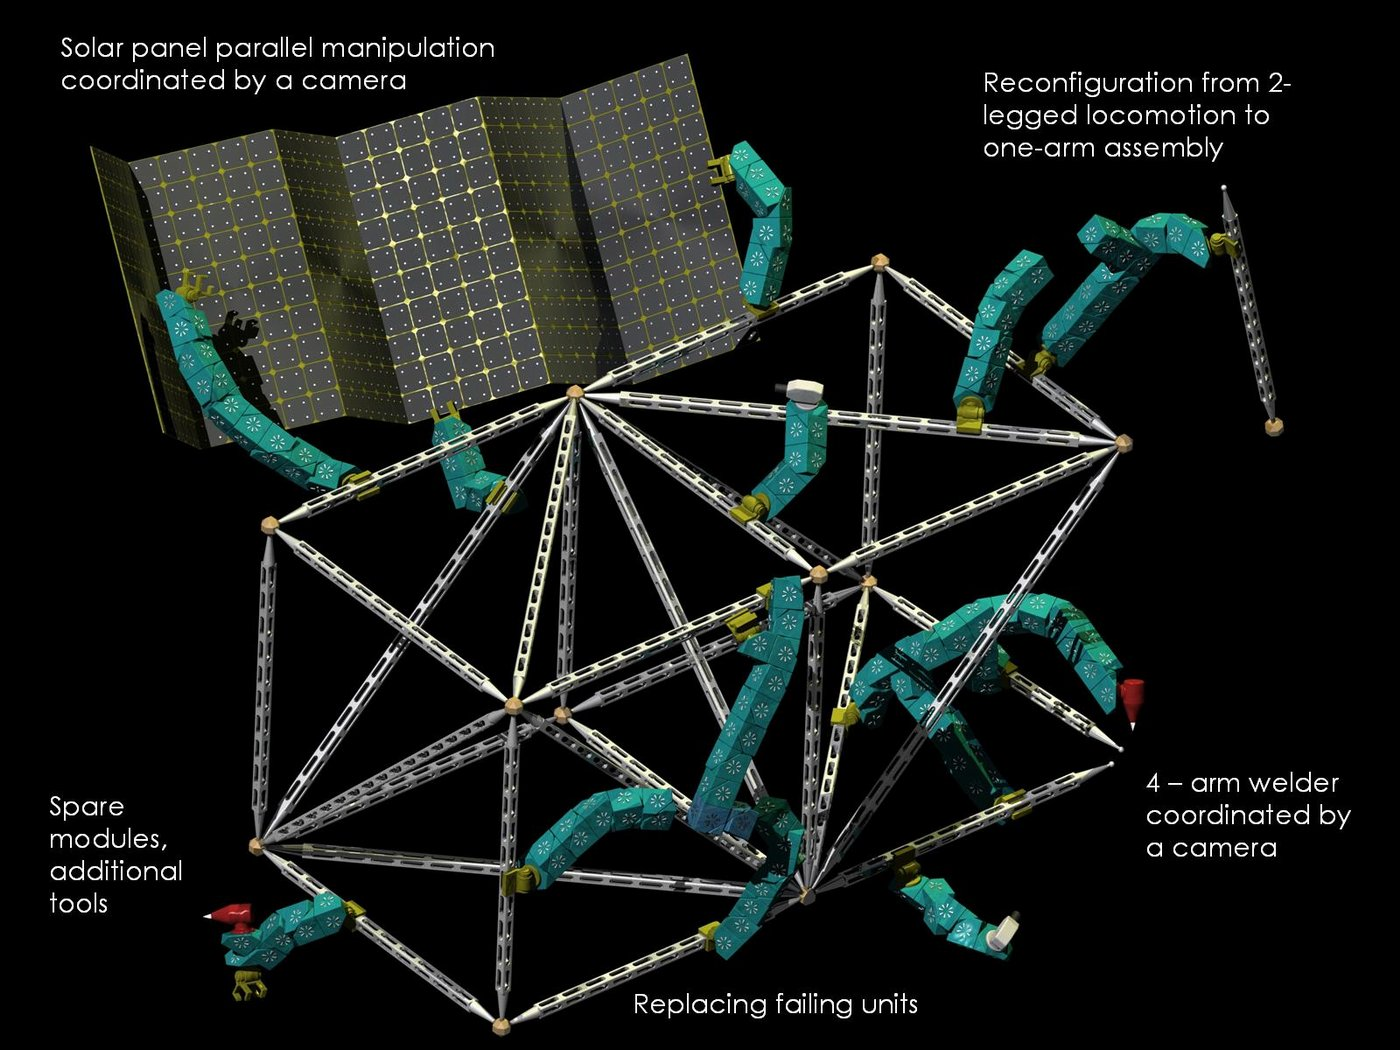
\includegraphics[width=\textwidth]{images/Intro_molecubes.jpg}
                \caption{Space applications.}
                \label{fig:intro_space_applications}
        \end{subfigure}
        \caption{Typical applications of modular robots.}
        \label{fig:intro_applications}
\end{figure}

In homogeneous modular robots, mass production can lower the cost of the robots, as they are all identical. But as currently these robots are used mainly for research, they are not mass produced, and usually very small batches of prototypes are manufactured. As each module is an autonomous robot, and therefore they need to have their own controller hardware and software, actuators (like motors), sensors, communication hardware and batteries, modular robots are usually very expensive, the cost of one single module has to be multiplied several times, increasing rapidly the cost of the robot.\\

Despite their versatility in uncertain situations, due to the high number of modules that compose a modular robot, they are usually hyper-redundant robots, robots with a large or infinite number of degrees of freedom. This complicates the search for adecuate locomotion gaits due to the increase in complexity to find the inverse kinematics of the robots, as well as the increase in difficulty of coordinating the movement of all the joints. \\

Other problem that arises in modular robotics is the distributed nature of the system, that requires each module to have its own controller, which has to interact with the other modules controllers in order to achieve a correct and optimal behavior of the whole modular robot. In this aspect, having a homogeneous controller (i.e. all the modules share exactly the same controller) eases the development and mainteinance of the controller, but a proper, scalable controller and communication protocol is still required for collaboratively control the entire robot.\\

In this thesis we address those three problems described: locomotion gait generation on a modular robot, designing a homogeneous distributed controller that can control the whole modular robot selecting the most appropiate gait for each configuration, and the development of a cheap and simple modular robot platform to test and validate locomotion gaits and controllers.\\ 

\section{Objectives}
\label{introduction_objectives}

The main objective of this thesis is to solve some of the problems in modular robotics mentioned in the introductory section. More precisely, to develop a homogeous distributed controller and optimal locomotion gaits that allow a modular robot to move as fast as possible adapting its gaits to its current configuration, and test this controller on both a simulated and a real modular robotic platform.\\

In order to achieve that objective successfully, we have divided it into four main objectives:
\begin{enumerate}
	\item \textbf{To find optimal locomotion gaits} for at least three different modular robot configurations by means of stochastic optimization algorithms.\\
	
	\item \textbf{To develop a homogeneous, distributed controller and communication algorithm} that allows a modular robot to discover its current configuration and select the most suitable gait for that configuration. \\	

	\item \textbf{To develop a software framework} that allows to simulate the modular robot and test the obtained optimal gaits, as well as the homogenous controller for their validation. This framework should be flexible enough to serve as a base for the development and testing of other controllers and configurations in the future.\\
	
	\item \textbf{To develop a cheap hardware platform} for testing the obtained optimal gaits and the distributed controller on the real world. This includes the design of both the mechanical part of the module as well as the control electronics, and the later assembly of the different configurations of the modular robot. This platform should also be upgradeable and reusable in future research related to modular robots.\\
\end{enumerate}

\newpage
\section{Phases of the project}
\label{introduction_phases}

\noindent
A brief description of the different phases of this project is presented here chronologically ordered:

\begin{enumerate}
	\item \textbf{Study of the existing work on the topic.}
		\begin{enumerate}
			\item Study of the state of the art on modular robotics.
			\item Test existing open source modular robotics platforms.
			~\\
		\end{enumerate}
		
	\item \textbf{Development of basic software framework for simulation.}
		\begin{enumerate}
			\item Development of basic digital model of the module to be used.
			\item Select and setup simulator.
			\item Development of the basic software for the control of the modular robot on the simulation.
			~\\
		\end{enumerate}				
		
	\item \textbf{Optimization of modular robot gaits.}
		\begin{enumerate}
			\item Study and selection of stochastic optimization algorithm to be used.
			\item Optimization of gaits for the main configurations to be studied.
			~\\
		\end{enumerate}
	
	\item \textbf{Development of the distributed control algorithm.}
		\begin{enumerate}
			\item Develop the theoretical distributed control algorithm for configuration discovery and gait selection.
			~\\
		\end{enumerate}
		
	\item \textbf{Development of the remaining software framework for testing the gaits and distributed controller.}
		\begin{enumerate}
			\item Development of the software related to the communication between modules.
			\item Development of the distributed controller for the module.
			\item Testing of the controller and gaits on the simulated modular robot.
			~\\
		\end{enumerate}

	\item \textbf{Development of the hardware platform for testing the gaits and distributed controller.}
		\begin{enumerate}
			\item Design, manufacturing and assembly of the control board.
			\item Design, manufacturing and assembly of the mechanical module.
			\item Assembly of the different modular robot configurations.
			\item Test of the locomotion gaits and distributed controller on the physical modular robot.
			~\\
		\end{enumerate}
		
	\item \textbf{Results documentation}
		\begin{enumerate}
			\item Comment and document software.
			\item Upload software and hardware designs to online repositories under a open source license.
			\item Write and defend thesis.
		\end{enumerate}
		
\end{enumerate}